%
% aufgaben.tex -- Kurzbeschreibungen der Aufgabenstellungen fuer die
%                 Seminar-Arbeiten
%
% (c) 2013 Prof Dr Andreas Mueller, Hochschule Rapperswil
% $Id$
%
\documentclass[a4paper,12pt]{article}
\usepackage{german}
\usepackage{amsmath}
\usepackage{amssymb}
\usepackage{amsfonts}
\usepackage{amsthm}
\usepackage{graphicx}
\usepackage{fancyhdr}
\usepackage{textcomp}
\usepackage[all]{xy}
\usepackage{txfonts}
\usepackage{alltt}
\usepackage{verbatim}
\usepackage{paralist}
\usepackage{makeidx}
\usepackage{array}
\usepackage{hyperref}
\begin{document}
\title{Aufgabenstellungen f"ur das Seminar\\``High Performance Computing''}
\author{Andreas M"uller\footnote{
University of Applied Sciences, Oberseestrasse 10, CH-8640 Rapperswil,
Switzerland, Email: {\tt andreas.mueller@hsr.ch}}}
\date{}
\maketitle
\section{Ziele des Seminars}
\begin{itemize}
\item
\item
\item
\item
\end{itemize}

\section{Auftrag}
Jeder Seminarteilnehmer bearbeitet ein Thema aus dem Bereich des
High Performance Computing,
stellt seine Resultate in Form eines
kurzen Papers (wenige Seiten) zusammen und stellt sie ausserdem
in Form einer Pr"asentation im Klassenrahmen vor.

Im Idealfall l"asst sich Ihr Paper fast unver"andert als Abschnitt
in das Skript aufnehmen, so dass den Teilnehmern am Ende des Seminars
ein kleiner ``Leitfaden zum High Performance Computing'' zur Verf"ugung steht,
der als Einstieg in die Fachliteratur dienen kann.
Das Skript im Source Code wird als Creative Commons Projekt auf
Github gefuhrt, unter dem URL
{\tt https://github.com/AndreasFMueller/SeminarHPC.git}.

Die Pr"asentation sollte nicht nur einfach den Stoff vorf"uhren,
sondern sollte gen"ugend Zahlenbeispiele, Aufgaben oder von Hand
durchf"uhrbare Schritte einhalten, dass die Zuh"orer sich durch
die Probleml"osung durcharbeiten und so ihr Verst"andnis des
Stoffes vertiefen k"onnen. Die Pr"asentation soll sich auch darum
bem"uhen, den Zusammenhang mit den anderen im Seminar behandelten
Themen herzustellen, also zum Beispiel darlegen, warum eine bestimmte
Methode in gewissen F"allen einer anderen, von jemand anderem behandelten
Methode vorzuziehen ist.

Die Darstellung soll vor allem verst"andlich und anschaulich
sein, aber nat"urlich auch so exakt wie m"oglich.
Sie muss alllerdings nicht die strengen Anforderungen an einen
vollst"andigen Beweis erf"ullen. Es ist besser, sich auf die
wesentlichsten F"alle zu beschr"anken, oder die Methode mit
einem niedrigdimensionalen Beispiel zu illustrieren, welche
die Methode verst"andlich macht, als den Zuh"orer mit stundenlangen
Falldiskussionen zu langweilen.

\section{Aufgaben}
Die nachstehend skizzierten Aufgaben werden in dieser Reihenfolge im
Seminar behandelt. Die genauen Termine werden sp"ater bekannt
gegeben. Als Faustregel dient, dass Aufgabe Nummer $n$ in der Woche
$n + 2$ behandelt wird.

\newtheorem{aufgabe}{Aufgabe}

\begin{aufgabe}
Beschleunigung der R"uckprojektion in einem CAT Scanner.
\end{aufgabe}

Eine CAT Scanner oder Computer-Tomograph ist in der Lage, aus
einzelnen linearen R"ontgenbildern in einer Ebene durch einen
K"orper ein Schnittbild durch den K"orper zu gewinnen.
CAT Scanner wurden in den 60er und 70er Jahren entwickelt
und haben die medizinische Diagnostik revolutioniert. 

Die mathematische Aufgabe hinter einem CAT Scanner kann wie folgt
beschrieben werden.
Wir m"ochten ein Schnittbild durch eine K"orper erstellen,
wir m"ochten also die Absorptionsdichte in Abh"angigkeit $f(x,y)$ von 
$x$ und $y$ ermitteln.
Zur Verf"ugung stehen uns R"ontgenbilder, die in verschiedenen Richtungen
aufgenommen wurden.
Der R"ontgenstrahl durch den Punkt $(r\cos\vartheta, r\sin\vartheta)$
mit der Normalen $(\cos\vartheta,\sin\vartheta)$ wird abh"angig
von $f$ abgeschw"acht, die 
gesamte Absorbtion entlang dieses Strahls ist gegeben durch das
Integral entlang dieses Strahls.
Den Strahl kann man in Parameterdarstellung beschreiben:
\[
\begin{pmatrix}
r\cos\vartheta\\
r\sin\vartheta
\end{pmatrix}
+s
\begin{pmatrix}
-\sin\vartheta\\
\cos\vartheta
\end{pmatrix}
\]
Die aufgenommenen R"ontgenbilder haben also Absorbtionen
\[
{\cal R}f(r,\vartheta)=\int_{-\infty}^{\infty}
f(r\cos\vartheta-s\sin\vartheta, r\sin\vartheta+s\cos\vartheta)\,ds.
\]
Die Funktion ${\cal R}f(r,\vartheta)$ heisst die Radon-Transformierte
von $f$, nach Johann Karl August Radon (1887--1956), der diese Transformation
bereits 1917 studiert hat.

Die Aufgabe eines Computer-Tomographen ist also, aus ${\cal R}f$ die
urspr"ungliche Funktion $f$ zu rekonstruieren.
Ein wesentlicher Schritt dazu ist die sogenannte R"uckprojektion.
Ziel dieser Aufgabe ist herauszufinden, wie gut sich die R"uckprojektion
mit Hilfe von Graphikkarten beschleunigen l"asst.

Um den Wert $f(x,y)$ zu finden, muss man sicher alle Werte von ${\cal R}f$
verwenden, die zu Geraden geh"oren, die durch den Punkt $(x,y)$ gehen.
Mittel man "uber alle Werte von ${\cal R}f(r,\vartheta)$, die zu 
Geraden durch $(x,y)$ geh"oren, dann werden sich die Werte von anderen
Pixeln ausmitteln zu einem mittleren Wert. Man kann sogar eine
Formel daf"ur angeben:
\[
{\cal B}g(x,y)
=
\frac1\pi\int_0^\pi g(x\cos\vartheta+y\sin\vartheta,\vartheta)\,d\vartheta.
\]
Diese R"uckprojektion ist also eine erste, noch etwas verschleierte
N"aherung f"ur $f(x,y)$, durch weitere Verarbeitungsschritte, die
nicht Gegenstand dieser Aufgabe sind, kann man das Bild auch noch
scharf hinbekommen.

Literatur: Timothy G.~Feeman, {\it The Mathematics of Medical Imaging:
A Beginners Guide}, Springer Undergraduate Texts in Mathematics and
Techology, 2010.


\begin{aufgabe}
Masssiv-paralleles DES Cracking
\end{aufgabe}

Im Compute Server der Gruppe Mathematik stehen 4 8-core CPUs mit
64GB RAM und 4 Nvidia Tesla Karten zur Verf"ugung.
Jede der im Skript vorgestellten Technologien k"onnte verwendet
werden, um Brute Force DES cracking zu implementieren.
Der Inhalt dieser Aufgabe ist eine M"oglichkeit zu finden: alle
Resourcen der Maschine vollst"andig auszunutzen.


M"oglicher Ausgangspunkt:
Source Code eines Studentenprojektes an der Purdue University mit
einer OpenCL Implementation f"ur DES:
\url{https://www.dropbox.com/s/hnqxmdd1yks6xnd/Research.zip}

\begin{aufgabe}
SOR und SSOR: Konvergenzbeschleunigung f"ur iterative Solver f"ur
lineare Gleichungssysteme.
\end{aufgabe}

Im Skript werden der Jacobi- und der Gauss-Seidel-Algorithmus
behandelt. Mit Hilfe von Matrixzerlegungen wurde gezeigt, wie man
die Konvergenzgeschwindigkeit ermitteln kann. Successive OverRelaxation
(SOR) und Symmetric SOR (SSOR) sind Methoden, die Konvergenz zu
beschleunigen.

Ziel dieser Aufgabe ist an Beispielen und mit theoretischen 
"Uberlegungen zu zeigen, wie SOR die Konvergenz beschleunigt.

Literatur: David S.~Watkins, {\it Fundamentals of Matrix Computations},
Wiley, 2010 (in der HSR Bibliothek).

\begin{aufgabe}
Als Motivationsbeispiel im Abschnitt "uber iterative Methoden f"ur lineare
Gleichungssysteme wurde die partielle Differentialgleichung mit
\[
\Delta u = f(x,y)
\]
Randbedingungen $u(x,y)=g(x,y)$ f"ur $(x,y)\in\partial\Omega$ dargestellt.
Man finde eine m"oglichst effiziente numerische L"osung f"ur dieses Problem.
\end{aufgabe}

Die Diskretisierung f"uhrt auf ein Gleichungssystem mit der Matrix
\[
A=\begin{pmatrix}
T&E& & &      & \\
E&T&E& &      & \\
 &E&T&E&      & \\
 & &E&T&      & \\
 & & & &\ddots& \\
 & & & &      &T
\end{pmatrix}
\]
Zerlegt man die Matrix als
\[
A
=
\underbrace{
\begin{pmatrix}
T& & & &      & \\
 &T& & &      & \\
 & &T& &      & \\
 & & &T&      & \\
 & & & &\ddots& \\
 & & & &      &T
\end{pmatrix}}_M
+
\underbrace{
\begin{pmatrix}
0&E& & &      & \\
E&0&E& &      & \\
 &E&0&E&      & \\
 & &E&0&      & \\
 & & & &\ddots& \\
 & & & &      &0
\end{pmatrix}}_N,
\]
erh"alt mein ein interatives Verfahren.
Die Matrix $M$ ist tridiagonal, diese spezielle Form einer Matrix ist
besonderes effizient invertierbar in Zeit $O(n)$.
Ausserdem ist
\[
M^{-1}=\begin{pmatrix}
T^{-1}&      &      \\
      &\ddots&      \\
      &      &T^{-1}
\end{pmatrix},
\]
Die Inverse von $M$ ist also sehr einfach aufgebaut,
insbesondere gibt es in der LAPACK-Library eigene Funktionen zur 
Invertierung solcher Matrizen.
Damit wird die Iterationsgleichung
$ x=M^{-1}(b - Nx)$
effizient implementierbar.

Vergleichen Sie die Performance dieses Verfahrens mit den Standard-Verfahren
von Jacobi und Gauss-Seidel.
Es ist auch denkbar, als Erweiterung den dreidimensionalen Fall zu untersuchen.

\chapter{Visualisierung der Greenschen Funktion}
\rhead{Visualisierung der Greenschen Funktion}
\begin{refsection}
\chapterauthor{Andreas Linggi, Stefan Steiner}

\section{Aufgabenstellung}

Um ein Problem der Mathematik besser zu verstehen, ist es oft sehr
hilfreich, wenn es verst"andlich beschrieben ist. Eine Visualisierung
in Form eines Bildes oder kurzen Films ist dabei eine M"oglichkeit,
dies zu bewerkstelligen.
	
Ziel dieses Projektes war, die Greensche Funktion in zwei Dimensionen
zu visualisieren. Die L"osung f"ur eine Dimension wurde bereits in
einem kurzen Film veranschaulicht
\footnote{\url{https://www.youtube.com/watch?v=Wpi7Gf7V2HY}}. Es
soll dabei zuerst eine partielle Differentialgleichung gel"ost und
danach visualisiert werden. Die Greensche Funktion erm"oglicht die
Berechnung eines Problems durch Superposition. Darum sollten auch
verschiedene Anfangswerte untersucht werden und wie diese sich auf
die L"osungen auswirken.
	
Als Differentialgleichung ist das Potentialproblem vorgegeben.
Gegeben ist eine leitende Platte, die am Rande geerdet sei. Wenn
nun ein Potential an einem oder mehreren Punkten auf dieser Platte
anliegt, ist es von Interesse zu wissen, welches Potential man nun
an einem beliebigen Punkt auf der Platte misst.

\section{George Green}

Der Namensgeber f"ur die Greensche Funktion ist George Green. Er
war ein britischer Physiker und Mathematiker. Geboren wurde er 1793
in der N"ahe von Nottingham. Sein Vater betrieb eine M"uhle und
George Green arbeitete ebenfalls als M"uller. Nach dem Tod seines
Vaters f"uhrte er den M"uhlenbetrieb fort. Bemerkenswert ist, dass
Green nur etwa zwei Jahre in die Schule ging. Mathematische und
Physikalische Grundlagen brachte er sich selber bei. Der Ort an dem
er lernte war seine M"uhle. Da nie ein Portrait von ihm angefertigt
wurde, gibt es kein Bild von ihm. Darum wird anstatt seinem Konterfei
jeweils eine Windm"uhle verwendet um ihn darzustellen. Die Windm"uhle
gibt es "ubrigens immer noch. Green ver"offentliche mit etwa dreissig
Jahren seine erste Arbeit. Diese wurde kaum beachtet, ausser von
einem adligen Mathematiker namens Sir Edward Bromhead. Er ermutigte
Green, im Alter von vierzig Jahren, in Cambridge zu studieren.
Interessant zu wissen ist dazu, dass dort zu dieser Zeit die Theorien
von Laplace und Fourier noch nicht gelehrt wurden. Green hatte sich
jedoch durch diese Theorien gelesen und sogar noch einige Erweiterungen
hinzugef"ugt. Vier Jahre nachdem er graduierte und kurz vor seinem
internationalen Durchbruch stand, starb er 1841 jedoch an einer
schweren Grippe. Dadurch geriet seine Arbeit f"ur einige Zeit in
Vergessenheit.
	
George Green ist besonders bekannt f"ur das Greensche Theorem und
die Greensche Funktion. Er besch"aftigte sich mit der L"osung von
partiellen Differentialgleichungen und stellte damit unter anderem
mathematische Hilfsmittel bereit, die sogar in der Quantenfeldtheorie
im 20. Jahrhundert von Bedeutung waren \cite{wiki:green}.
	
Neben vielen anderen Pers"onlichkeiten wie Maxwell, Dirac oder
Newton ist er in der Westminster Abbey in London mit einer Gedenktafel
verewigt \cite{wiki:westminster}. Der Grund, warum George Green nicht
so popul"ar ist wie Gauss oder Maxwell, liegt wahrscheinlich darin,
dass von seiner Zeit, als er in seiner M"uhle gearbeitet hat, wenig
bekannt ist. Auch war er nur f"ur sehr kurze Zeit in Cambridge
t"atig.

\begin{figure}                    
\centering 
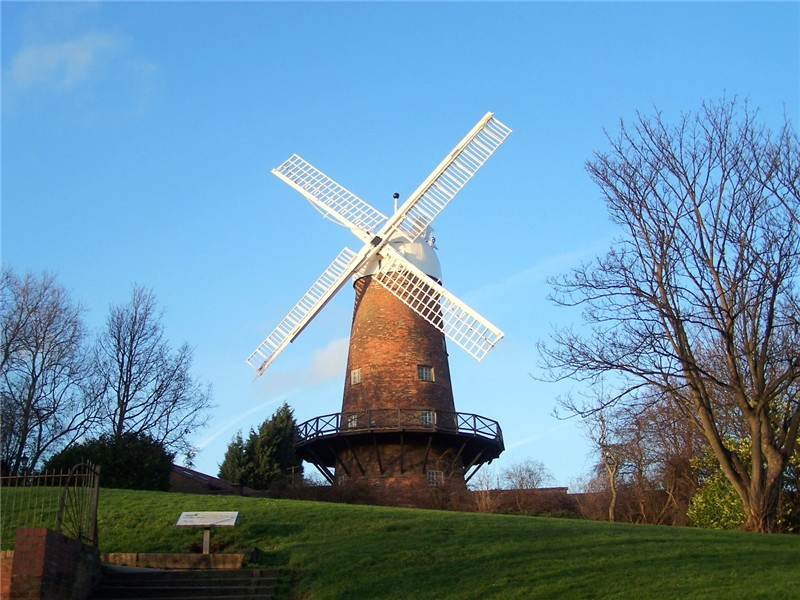
\includegraphics[width=\hsize]{green/images/greens_windmill.jpg} 
\caption{Windm"uhle, in der Green f"ur lange Zeit gearbeitet hat} 
\label{fig:abb1} 
\end{figure} 
	
\section{Algorithmus}
Um eine Visualisierung "uberhaupt durchf"uhren zu k"onnen, braucht
es in unserem Fall Daten, mit denen wir arbeiten k"onnen. Diese
liefert uns ein Programm, bei welchem wir Daten einspeisen und im
Gegenzug bearbeitet erhalten.
	
Das Problem, welches wir hier l"osen, wurde ebenfalls von Philip
Solenthaler und Reto Christen bearbeitet. Sie haben untersucht, wie
ein Programm geschrieben werden kann, welches dieses Problem
m"oglichst effizient l"ost.

\subsection{Mathematischer Ansatz zur L"osung}

Das Potentialproblem auf der leitenden Platte, welches wir l"osen
m"ochten, hat nun folgende partielle Differentialgleichung:
\begin{equation}\label{eq:gleichung}
\dfrac{\partial^2 u}{\partial x^2}+\dfrac{\partial^2 u}{\partial y^2} = f(x,y).
\end{equation}
Wobei die Rand-, und Anfangsbedingungen auf der leitenden Platte alle null sind. 
	
Die quadratische Platte mit der L"ange $n\times n$ wird dabei mit
den Werten $u_{ij}$ diskretisiert, wobei $0 < i,j<n$. Wir bekommen
eine endliche Anzahl an Werte $u$.
%	 Dabei wird f"ur jeden Wert $u$ diese Gleichung gel"ost. 
Der Ansatz f"ur eine L"osung dieses Problems bietet die lineare
Algebra, welcher bereits im Theorieteil des Skriptes ausf"uhrlich
hergeleitet wird. Das bedeutet, wir m"ussen ein Problem folgender
Art l"osen.
\begin{equation}
Au = f
\end{equation}
Es sei dabei $A$ die Koeffizientenmatrix, $f$ der St"orvektor und
$u$ der L"osungsvektor.
	
Die leitende Platte wird als eine Fl"ache visualisiert. Um diese
als Vektor $u$ zu schreiben ist dabei festgelegt worden, dass die
Spalten dieser diskretisierten Fl"ache untereinander geschrieben
werden. Dies ergibt Vektoren der l"ange $n^2$.
	
Aus diesem Zusammenhang heraus ergibt sich dabei die Koeffizientenmatrix
$A$.
\[
	A=\left(
	\begin{array}{ccccc|ccccc|c|ccccc}
	    -4&     1&     0&\cdots&     0 &     1&     0&     0&\cdots&     0 &\cdots &      &      &      &      &      \\
	     1&    -4&     1&\cdots&     0 &     0&     1&     0&\cdots&     0 &\cdots &      &      &      &      &      \\
	     0&     1&    -4&\cdots&     0 &     0&     0&     1&\cdots&     0 &\cdots &      &      &     0&      &      \\
	\vdots&\vdots&\vdots&\ddots&\vdots &\vdots&\vdots&\vdots&\ddots&\vdots &       &      &      &      &      &      \\
	     0&     0&     0&\cdots&    -4 &     0&     0&     0&\dots &     1 &\cdots &      &      &      &      &      \\
	\hline
	     1&     0&     0&\cdots&     0 &    -4&     1&     0&\dots &     0 &\cdots &      &      &      &      &      \\
	     0&     1&     0&\cdots&     0 &     1&    -4&     1&\dots &     0 &\cdots &      &      &      &      &      \\
	     0&     0&     1&\cdots&     0 &     0&     1&    -4&\dots &     0 &\cdots &      &      &     0&      &      \\
	\vdots&\vdots&\vdots&\ddots&\vdots &\vdots&\vdots&\vdots&\ddots&\vdots &       &      &      &      &      &      \\
	     0&     0&     0&\cdots&     1 &     0&     0&     0&\cdots&    -4 &\cdots &      &      &      &      &      \\
	\hline
	\vdots&\vdots&\vdots&      &\vdots &\vdots&\vdots&\vdots&      &\vdots &\ddots &\vdots&\vdots&\vdots&      &\vdots\\
	\hline
	      &      &      &      &       &      &      &      &      &       &\cdots &    -4&     1&     0&\cdots&     0\\
	      &      &      &      &       &      &      &      &      &       &\cdots &     1&    -4&     1&\cdots&     0\\
	      &      &     0&      &       &      &      &     0&      &       &\cdots &     0&     1&    -4&\cdots&     0\\
	      &      &      &      &       &      &      &      &      &       &       &\vdots&\vdots&\vdots&\ddots&\vdots\\
	      &      &      &      &       &      &      &      &      &       &\cdots &     0&     0&     0&\cdots&    -4\\
	\end{array}
	\right) 
	\]

\subsection{Technische Umsetzung}

Die Matrix $A$ enth"alt die Koeffizienten f"ur die partielle
Differentialgleichung der zweiten Ordnung. Sie hat die Gr"osse $n^2
\times n^2$. Diese Matrix im Arbeitsspeicher abzuspeichern w"are
f"ur mittelgrosse Matrizen schon nicht mehr
m"oglich \cite{mueller:hpcseminar}.
	
Der ben"otigte Speicher f"ur eine Platte mit der Gr"osse $500 \times
500$ und \verb|float| Werten (4 Byte) w"are
	
\begin{equation}
500^2 \times 500^2 \cdot 4\;\mathrm{Byte} = 232.8\;\mathrm{GByte}
\end{equation}
	
Mit $n = 1000$ sogar 3.64\,TByte, also definitiv zu viel. Dies ist
aber auch gar nicht n"otig. Es m"ussen jeweils nur die Nachbarelemente
von $u_{ij}$ addiert und durch einen konstanten Faktor geteilt
werden, die Randelemente sind dabei Null zu setzen.

\begin{eqnarray}
%		f_{ij} = u_{i-i,j}+u_{i+1,j}+u_{i,j+1}+u_{i,j-1}-4u_{ij}\\
u_{ij} = \dfrac{u_{i-i,j}+u_{i+1,j}+u_{i,j+1}+u_{i,j-1}-f_{ij}}{4}
\label{eq:gauss-seidel}
\end{eqnarray}
	
Da die diskretisierte partielle Ableitung jeweils nur die Elemente
ober/unterhalb und links/rechts des aktuellen Elementes in die
Rechnung mit einbezieht (\ref{eq:gauss-seidel}), m"ussen mindestens
$n$ Iterationen durchgef"uhrt werden, damit sich das Potential "uber
die ganze Ebene verteilt.
	
\subsubsection{Parallelisierung}
	
Um das Gleichungssystem (\ref{eq:gleichung}) zu l"osen, haben wir
den Gauss-Seidel Algorithmus benutzt. Bei diesem Algorithmus ist
die aktuelle Zeile von der vorherigen abh"angig. Bei der Parallelisierung
wird das Gleichungssystem an verschiedenen Stellen zu l"osen begonnen.
Das ist zwar nicht so effizient, wie ein "'normaler"' Gauss-Seidel,
wird aber durch die Parallelisierung schneller.
		
Die Abweichung ist bei den ersten Schritten am gr"ossten, und wird
bei jeder Iteration kleiner. Als wir die ersten Berechnungen durch
gef"uhrt hatten, fiel uns auf, dass die einzelnen Threads am Anfang
gut als Linien von Spitzen sichtbar sind (\ref{fig:201_1}).
		
\begin{figure}
\centering
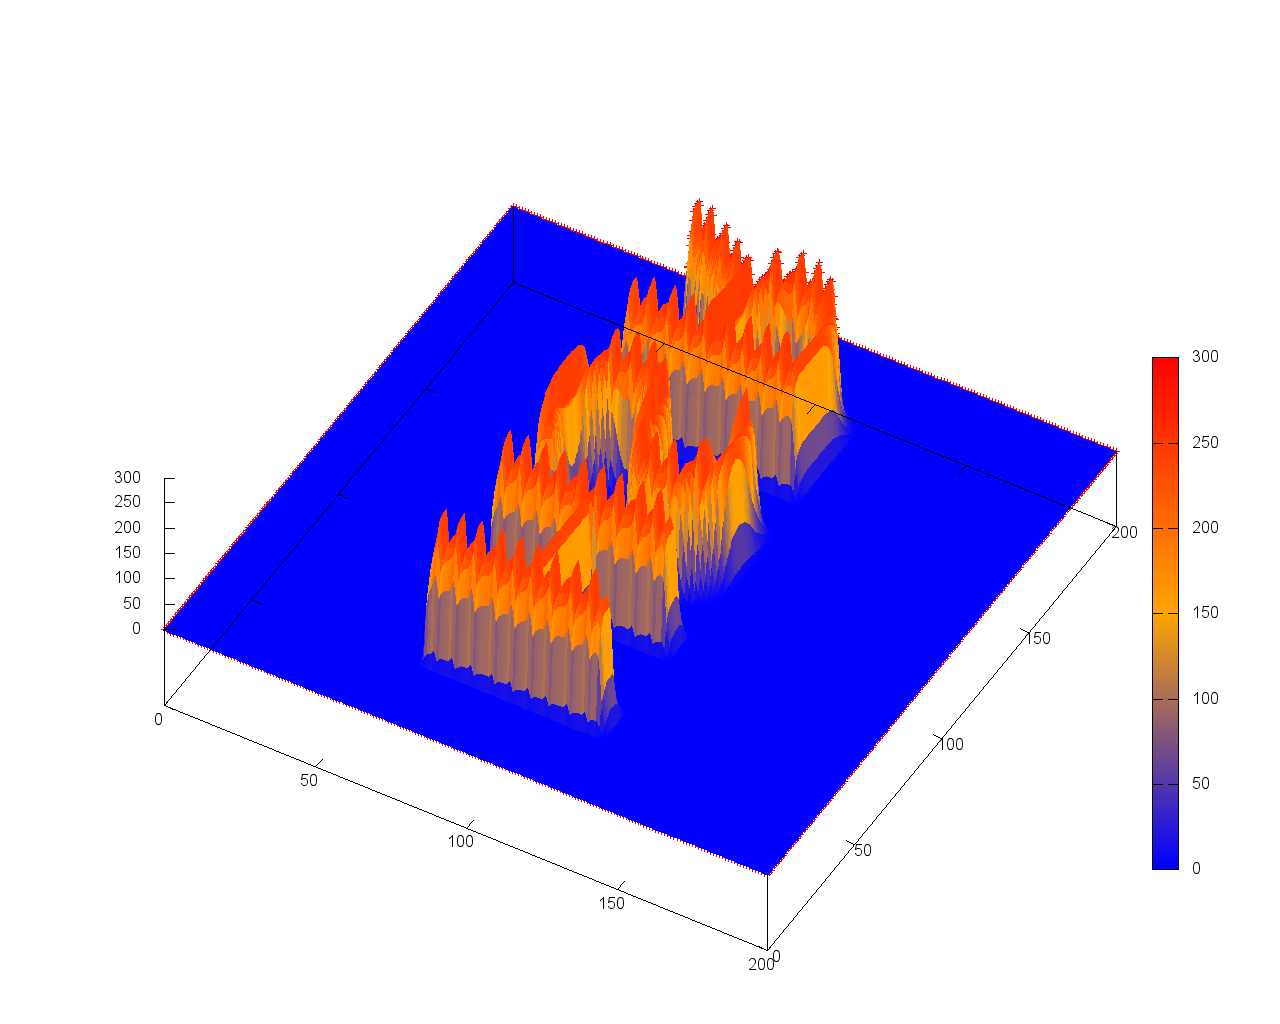
\includegraphics[width=\hsize]{green/images/step001}
\caption{Berechnung von einer $201 \times 201$ Fl"ache mit 32 Threads
nach dem ersten Iterationsschritt}
\label{fig:201_1}
\end{figure}
		
		
Wir haben uns f"ur Open-MP entschieden, da es f"ur uns die einfachste
Methode war, die Berechnung zu parallelisieren. Wie bei der Arbeit
von Christen und Solenthaler erkl"art, w"are Open-MPI die effizienteste
Weise, um solch ein Problem zu l"osen. Da hier nur die Resultate
des Algorithmus von Interesse waren und wir relativ kleine Probleme
gel"ost haben, hat es sich nicht gelohnt, den Mehraufwand f"ur
Open-MPI zu betreiben. Die Rechenzeit war absolut im Rahmen.
		
Wie schon beim Kugelsternhaufen erw"ahnt, ist nun diese Open-MP
Parallelisierung einfach zu realisieren, wie folgendes Beispiel
zeigt.
		
\begin{code}
// Parallelisierung einer for-Schleife
	int numthreads = 32;
	#pragma omp parallel for num_threads(numthreads)
		for (i = 0; i < dim; i++)
		{ ...
\end{code}

\subsubsection{Dateiformate}
	
Um mit der Datenflut umgehen zu k"onnen, musste ebenfalls eine
L"osung entwickelt werden. Als Eingabedatei wurde ein Bild im FITS
Format verwendet. Da es jedoch einfacher schien, wurde w"ahrend des
Programmes mit \texttt{.csv} Files gearbeitet. Dabei war der
technische Aufwand gering und die Resultate konnten schnell
kontrolliert werden. Aus diesen \texttt{.csv} Dateien kann mit GNU-Plot ein
Bild erstellt werden. Optional dienen diese als Vorlage f"ur einen
kurzen Film.

\section{Visualisierung}
	
\subsection{Prinzip}
			
Ziel der Visualisierung ist, die einzelnen Schritte einer Berechnung
mit der Greenschen Funktion zu zeigen. Bei jedem Schritt kommen
zus"atzliche Werte zum vorherigen Schritt hinzu. Die Bilder aus
\ref{fig:dreiSchritte} stellen drei solche Schritte dar, wie wir
sie in unserer Arbeit definiert haben.
		
W"urden wir jeweils die L"osungen f"ur alle Werte $u_{ij}$ einzeln
berechnen und sie dann addieren, m"ussten wir diese Schritte
schlussendlich noch visuell darstellen. Der Aufwand hierf"ur ist
aber betr"achtlich. Da die Darstellung im Vordergrund steht, ist das Verfahren zur
Berechnung irrelevant f"ur das Endergebnis. Um die Rechnung zu
beschleunigen, haben wir uns f"ur einen anderen Algorithmus
entschieden, welcher uns erlaubt, so viele Werte $u_{ij}$ wie n"otig
miteinander zu l"osen.
		
Wir werden dementsprechend immer das gleiche Problem l"osen mit
jeweils zus"atzlichen Werten $u$. Jeder dieser Schritte hat ein
Bild mit den vorherigen plus den neuen Werten zur Folge. Zusammengestellt
ergeben diese Bilder eine anschauliche Visualisierung der Greenschen
Funktion.
	
	
\subsection{Darstellungsm"oglichkeiten}
	
Welche Werte wir jeweils in einem Schritt dazu nehmen ist noch
offen. Man k"onnte beispielsweise die Fl"ache von oben links bis
unten rechts durchgehen und immer ein oder mehrere Punkte dazu
nehmen. Es ist auch vorstellbar, diese Punkte zuf"allig auszuw"ahlen,
bis alle Punkte berechnet wurden. Der Nachteil dieser Verfahren
ist, dass sie nicht viel weniger aufw"andig sind, als das Verfahren,
welches alle Punkte einzeln berechnet. Wenn beispielsweise eine
Fl"ache bzw. Bild mit $500 \times 500$ Werten berechnet werden soll,
muss das Problem 250\,000 mal vollst"andig gel"ost werden. Es w"aren
auch 250\,000 Bilder vorhanden, eine Datenflut, die unser Auge wohl
kaum bew"altigen kann. Es ist fraglich, wie sinnvoll eine solche
Visualisierung ist.
		
Um das zu verhindern, haben wir uns entschieden, in der Mitte einer
solchen Fl"ache zu beginnen und dann schrittweise, Ring f"ur Ring,
nach aussen zugehen.

\begin{figure}
\centering
\begin{tabular}{ccc}
\includegraphics[width=0.3\hsize]{green/images/resultate/grfl/step0057.png}
& \includegraphics[width=0.3\hsize]{green/images/resultate/grfl/step0111.png}
& \includegraphics[width=0.3\hsize]{green/images/resultate/grfl/step0144.png}
\end{tabular}		
\caption{Die Schritte 57, 111 und 144 auf einer Fl"ache, die durch
$500 \times 500$ Werte dargestellt wird.}
\label{fig:dreiSchritte}
\end{figure}
	
In jedem dieser drei Schritte werden nur die roten Punkte in die
Berechnung ber"ucksichtigt, die anderen werden gleich Null gesetzt.
Jeder Schritt wird vollst"andig gel"ost, bis der maximale Fehler
eine Grenze unterschreitet.
	
\subsection{Technische Umsetzung}
	
Vor jeder dieser Berechnungen wird ein Vektor $f$, der unsere Fl"ache
repr"asentiert, so manipuliert, dass der helle "aussere Bereich
gleich Null gesetzt wird. Danach wird die Berechnung, die in jedem
Schritt identisch ist, durchgef"uhrt.
		
Wir speichern den berechneten Vektor $u$ als Matrix in einem \texttt{.csv}
File mit einer Genauigkeit von vier Nachkommastellen ab, was f"ur
eine Visualisierung gen"ugt. Anfangs benutzten wir MATLAB um aus
dem \texttt{.csv}-File eine anst"andige Visualisierung zu erhalten. Der
Aufwand war gering und die Resultate waren schnell kontrollierbar.
		
\lstinputlisting{green/csvToMatrixAndPlot.m}
		
Um das zu automatisieren benutzen wir sp"ater Gnuplot, welches sich
mit C-Code ohne Probleme ansprechen l"asst und uns die Bilder
automatisch mit dem vorgegebenen Einstellungen erstellt.
		
fmt: standard input: Illegal byte sequence
Gnuplot ist ein Kommandozeilen basiertes OpenSource Tool, das aber
auch mit GUI erh"altlich ist.
		
\lstinputlisting{green/gnuplot.c}
	
\subsection{Generieren der Bilder}
	
Die Bilder werden, nachdem alle Einzelschritte berechnet wurden, aus
den Dateien wiederum parallelisiert in einer \verb|for|-Schleife
zu \texttt{.png} Bilddateien verarbeitet. Da der letzte Schritt das Maximum
bzw. Minimum aller Schritte enth"alt, sofern wir nur Potentiale mit
gleichen Vorzeichen haben, wird die Skalierung der $z$-Achse direkt
aus diesen Daten berechnet. Dies garantiert und eine optimale
Darstellung.
		
Wir haben jeweils zwei verschiedene Ansichten erstellt: Eine normal
Ansicht, d.h ein 3D-Plot wie er z.~B.~in \ref{fig:201_1} zusehen
ist und eine Ansicht von oben mit H"ohenlinien. Aus den Bilddateien
wird am Schluss optional noch ein Video erstellt.
		
\section{Probleme}

\subsection{Konvergenz}
	
Wir haben anfangs den HSR-Schriftzug als FITS-File in eine Matrix 
eingelesen und diesen als Vektor $f$ abgespeichert. Der maximale
Wert des L"osungsvektors $u$ betrug anfangs nur 255, stieg nach
einigen hundert Iterationen auf "uber 3000 an und die Funktion nahm
die Form eines Haufens an. Wir hatten mit einem anderem Resultat
gerechnet und "uberpr"uften unseren Algorithmus. Wir entdeckten
keinen Fehler in unserem Algorithmus und konnten die Werte mit
MATLAB verifizieren. Die n"achste Frage war, ob der Gauss-Seidel
Algorithmus konvergiert. Wir berechneten den Spektralradius der
Matrix $A$ gem"ass Definition\;5.1 aus dem Skript
HPC\cite{mueller:hpcseminar}:
	
\begin{eqnarray}
A = M+N\\
\varrho(M^{-1}N)<1
\end{eqnarray}
		
Die Gr"osse der Matrix $A$ nimmt mit $n^4$ zu, weshalb die Berechnung
der Spektralradien mit MATLAB sehr schnell rechenaufw"andig wird.
Darum haben wir nur Spektralradien mit kleinem $n$ berechnet.
		
\begin{table}
\begin{tabular}{cc}
n & Specktralradius $\varrho$\\\hline
5 & 0.7500\\
10 & 0.92063\\
15 & 0.96194\\
20 & 0.97779\\
25 & 0.98547\\
40 & 0.99414
\end{tabular}
\centering
\caption{Spaktralradien der Matrix $A$ f"ur eine Matrix $f$ mit der Gr"osse $n\times n$}
\end{table}
	
Einerseits sind alle Spaktralradien kleiner Eins, was gut ist,
andererseits sind sie sehr nahe bei Eins, was erkl"art wieso unser
Algorithmus so langsam konvergiert.
		
Wir hatten sp"ater Erfolge, wenn wir die Anfangswerte des Vektors
$f$ klein w"ahlten $(f_{ij}<1)$. So waren die Fehler von Anfang an
kleiner und wir bekamen brauchbare Werte.
	
\subsection{Datenflut}
	
Bei Platten mit feiner Diskreditierung mussten wir darauf achten,
dass wir nicht zu viele Daten abspeichern. Wir mussten das Programm
so umschreiben, dass wir einstellen konnten, wie viele Bilder wir
schlussendlich wollten. Anhand dieser Einstellung wurden nur
die ben"otigten \texttt{.csv} und \texttt{.png} Dateien abgespeichert.
Das Programm wurde dadurch automatisch auch gleich viel schneller.
		
\begin{beispiel}
Wir wollen eine Platte mit  $40 \times 40$ Werten berechnen. Um die
Konvergenz beobachten zu k"onnen, speichern wir nach jeder Iteration
die Werte in eine \texttt{.csv} Datei ab. Es sind etwa 3000 bis 4000 Iterationen
n"otig bis sich die Werte nicht mehr ver"andern. Das ist problemlos m"oglich.
			
Wir wollen mehr, eine Platte mit $500 \times 500$ Werten. Um hier
eine Konvergenz zu beobachten, sind etwa 160\,000 bis 180\,000
Iterationen n"otig, wie wir sp"ater herausgefunden haben. Das Ganze
ist nat"urlich stark vom Ausgangsbild abh"angig.

Eine \texttt{.csv} Datei ist dann etwa 1.8\,MB gross, d.~h.~wir wollen ca.~300\,GB
abspeichern. Dies ist m"oglich, sofern gen"ugen Platz vorhanden
ist. Das eigentliche  Problem ist aber, dass das Programm nur noch
mit Daten speichern besch"aftigt ist und kaum noch Zeit zum Rechnen
hat.
\end{beispiel}
	
\subsection{Geeigneter Vektor $f$ finden}\label{sec:geeignetesF}

Ein ganz anderes Problem war, ein geeignetes Bild f"ur die Platte zu finden.
Es sollte die "Uberlagerung der Werte gut zeigen. Wir versuchten
verschiedene Muster, von einem Schriftzug, einzelne Buchstaben bis
zu einzelnen Punkten. Bew"ahrt hat sich eine Spirale. Da wir von
innen nach aussen gehen, kommen immer wieder neue Werte an verschiedenen
Seiten hinzu. Da schlussendlich nur eine geringe Anzahl Punkte
vorhanden sind, wirkt die Visualisierung nicht "uberladen und ist
"ubersichtlich.
		
\section{Resultate}

Wir haben mehrere Platten mit unterschiedlichen Potentialverteilungen
und mit unterschiedlicher Anzahl Diskretisierungspunkten berechnet.
Je nach Ausgangsbild, welches unsere Potentialverteilung darstellt,
ist die Superposition mehr oder weniger gut erkennbar. Wie in
\ref{sec:geeignetesF} erw"ahnt, hat sich eine Spirale von Punkten
bew"ahrt, die wir hier anhand vier verschiedenen Schritten zeigen
wollen. Das erste Bild ist jeweils die Fl"ache f"ur den jeweiligen
Schritt. Alle Punkte haben das selbe Potential. Pro Bild f"uhrten
wir 180\,000 Iterationen durch.

\newlength\breite
\begin{figure}
\centering
\begin{tabular}{cc}
\includegraphics[width=0.48\hsize]{green/images/resultate/grfl/step0057.png}
& \includegraphics[width=0.48\hsize]{green/images/resultate/grfl/step0111.png}\vspace{1cm}\\
\includegraphics[width=0.48\hsize]{green/images/resultate/cp/step0057.png}
& \includegraphics[width=0.48\hsize]{green/images/resultate/cp/step0111.png}\vspace{1cm}\\
\includegraphics[width=0.48\hsize]{green/images/resultate/np/step0057.png}
& \includegraphics[width=0.48\hsize]{green/images/resultate/np/step0111.png}
\end{tabular}		
\caption{Visualisierung von Green's Function: Schritte 75 und 111 }
\end{figure}
	
\begin{figure}
\centering
\begin{tabular}{cc}
\includegraphics[width=0.48\hsize]{green/images/resultate/grfl/step0144.png}
& \includegraphics[width=0.48\hsize]{green/images/resultate/grfl/step0175.png}\vspace{1cm}\\
\includegraphics[width=0.48\hsize]{green/images/resultate/cp/step0144.png}
& \includegraphics[width=0.48\hsize]{green/images/resultate/cp/step0175.png}\vspace{1cm}\\
\includegraphics[width=0.48\hsize]{green/images/resultate/np/step0144.png}
& \includegraphics[width=0.48\hsize]{green/images/resultate/np/step0175.png}
\end{tabular}		
\caption{Visualisierung von Green's Function: Schritte 144 und 175 }
\end{figure}

\printbibliography[heading=subbibliography]
\end{refsection}

\chapter{L"osung der W"armeleitungsgleichung}
\lhead{W"armeleitungsgleichung}

\chapterauthor{Andreas M"uller}

\index{Warmeleitung@W\"armeleitung}
{\parindent0pt
Die W"armeleitungsgleichung ist die prototypische parabolische
partielle Differentialgleichung.
In diesem Kapitel werden die Eigenheiten ihrer numerischen L"osung
diskutiert.}

\section{Problemstellung}
\rhead{Problemstellung}
Die W"armeleitungsgleichung f"ur einen Stab
auf dem Interval $[0,1]$ ist die partielle Differentialgleichung
\begin{equation}
\frac{\partial u}{\partial t}=\frac{\partial^2 u}{\partial x^2}, \qquad
0<x<1,\;t>0.
\label{heat:pdgl}
\end{equation}
Der Stab soll an den Enden mit W"armereservoirs verbunden sein, die
die Temperatur an den Enden festlegen. Sie kann mit der Zeit varieren.
Dies wird ausgedr"uckt durch
Randbedingungen
\index{Randbedingung}
\begin{align}
u(t,0)&=g_0(t),
&
u(t,0)&=g_1(t),&t&>0.
\label{heat:rand}
\end{align}
Die L"osung wird festgegelegt durch die Temperaturverteilung zu Beginn,
also durch
\begin{align}
u(0,x)=f(x),\qquad 0<x<1.
\end{align}
Gesucht ist ein numerisches L"osungsverfahren, welches die
W"armeleitungsgleichung numerisch l"ost.

Eine interessante und unphysikalische Eigenschaft der W"armeleitungsgleichung
ist die Existenz von L"osungen mit unendlich schneller Wirkungsausbreitung.
Die Funktion
\begin{equation}
u(t,x)=\frac1{\sqrt{2t}}e^{-\frac{x^2}{4t}}
\label{heat:solution}
\end{equation}
hat die folgenden Ableitungen:
\begin{align*}
\frac{\partial u}{\partial x}&=
-
\frac{x}{2t}\frac1{\sqrt{2t}}
e^{-\frac{x^2}{4t}}
&
\frac{\partial^2 u}{\partial x^2}&=
\biggl(\frac{x^2}{4t^2}-\frac1{2t}\biggr)
\frac1{\sqrt{2t}}
e^{-\frac{x^2}{4t}}
\\
\frac{\partial u}{\partial t}&=
\biggl(\frac{x^2}{4t^2}-\frac1{2t}\biggr)
\frac1{\sqrt{2t}}
e^{-\frac{x^2}{4t}}
\end{align*}
Die Funktion $u$ ist also eine L"osung der W"armeleitungsgleichung
(\ref{heat:pdgl}).
F"ur $t\to 0$ strebt $u(t,x)$ gegen eine Dirac $\delta$-Funktion
im Punkt 0.
Dies bedeutet, dass W"arme, die zur Zeit $t=0$ nur im Punkte vorhanden
ist, unmittelbar danach f"ur alle $t$ in Form eines Wertes $u(t,x) > 0$
sp"urbar ist.
Die W"arme im Punkt $0$ hat sich also mit unendlich grosser Geschwindigkeit
ausgebreitet.

\section{Diskretisation\label{heat:section-diskretisation}}
\begin{figure}
\begin{center}
\includegraphics[width=0.70\hsize]{heat/heat-1.pdf}
\end{center}
\caption{Diskretisation der W"armeleitungsgleichung. 
Aus jeweils drei horizontal benachbarten Punkten k"onnen die zweiten
Ableitungen berechnet werden.
Zwei in $t$-Richtung benachbarte solche Werte ergeben einen Mittelwert,
der f"ur die zweite Ableitung im Punkt $(i+\frac12,j)$ (schwarz)
stehen kann. Die erste Ableitung nach $t$ in diese Punkt kann aus
dem Differenzenquotienten ermittelt werden. So entstehen lineare
Gleichungen, die jeweils drei benachbarte noch nicht bekannte
$u$-Werte (rot) mit bereits bekannten Werten (blau) vernk"upfen.
\label{heat:diskretisation1}}
\end{figure}
Zur Diskretisation w"ahlen wir im Gebiet $[0,1]\times \mathbb R_+$ ein
Gitter. 
Da $x$- und $t$-Richtung offensichtlich nicht symmetrisch sind,
lassen wir offen, welche Gitterkonstanten wir in diesen Richtungen
verwenden wollen, und nennen sie $h_x=1/n$ und $h_t$. 
Die Funktion $u(t,x)$ wird jetzt ersetzt durch die Werte von $u$ auf
den Gitterpunkten, wir schreiben
\[
u_{ij} = u(ih_t, jh_x),\quad i\ge 0, 0\le j \le n.
\]
Durch die Randbedingungen wird ein Teil dieser Variablen bereits
festgelegt:
\begin{align*}
u_{0j}&=f(jh_x)&1&\le x < n\\
u_{i0}&=g_0(ih_t)&i&>0\\
u_{i1}&=g_1(ih_t)&i&>0\\
\end{align*}
Die Diskretisation der Differentialgleichung verwendet die in
Abschnitt~\ref{section-motivation} beschrieben Methode.
Die zweite partielle Ableitung von $u$ nach $x$ im Punkt $(ih_t, jh_x)$ 
kann durch
\begin{equation}
\frac1{h_x^2}(u_{i,j-1}-2u_{ij}+u_{i,j+1})
\label{heat:2ableitung}
\end{equation}
approximiert werden.
F"ur die erste partielle Ableitung nach $t$ ist man versucht,
den Differenzenquotienten
\begin{equation}
\frac1{h_t}(u_{i+1,j}-u_{ij})
\label{heat:1ableitung}
\end{equation}
zu verwenden.
Dieser Differenzenquotient ist aber eher eine Approximation f"ur
$\partial u/\partial t$ im Punkt $((i+\frac12)h_t, jh_x)$,
nicht $(ih_t,jh_x)$, man kann ihn also nicht direkt mit der
Approximation (\ref{heat:2ableitung}) f"ur die zweite Ableitung
in Beziehung setzen.
Man kann aber durch Mittelwertbildung aus (\ref{heat:2ableitung}) f"ur
die Punkte $(ih_t, jh_x)$ und $((i+1)h_t, jh_x)$ einen N"aherungswert
f"ur die zweite Ableitung finden, der sich mit der Approximation
f"ur die ersten Ableitung (\ref{heat:1ableitung}) vergleichen l"asst,
n"amlich
\begin{align}
\frac12\biggl(
\frac1{h_x^2}(u_{i,j-1}-2u_{ij}+u_{i,j+1})
+
\frac1{h_x^2}(u_{i+1,j-1}-2u_{i+1,j}+u_{i+1,j+1})
\biggr)
&=
\frac1{h_t}(u_{i+1,j}-u_{ij})
\label{heat:diskret}
\end{align}
Wir stellen die Gleichung um, so dass der linken Seite nur die 
Variablen f"ur die Zeit $(i+1)h_t$ stehen, und rechts nur die
Variablen f"ur die Zeit $ih_t$:
\begin{align}
\frac1{2h_x^2}(u_{i+1,j-1}-2u_{i+1,j}+u_{i+1,j+1})-\frac1{h_t}u_{i+1,j}
&=
-\frac1{2h_x^2}(u_{i,j-1}-2u_{ij}+u_{i,j+1})-\frac1{h_t}u_{ij}
\notag
\\
\frac1{2h_x^2}u_{i+1,j-1}
-\biggl(\frac1{h_x^2}+\frac1{h_t}\biggr)u_{i+1,j}
+\frac1{2h_x^2} u_{i+1,j+1}
&=
-\frac1{2h_x^2}u_{i,j-1}
+\biggl(\frac1{h_x^2}-\frac1{h_t}\biggr)u_{ij}
-\frac1{2h_x^2} u_{i,j+1}
\label{heat:gleichung}
\end{align}
Dies ist eine lineare Gleichung f"ur die Variablen $u_{i+1,j}$.
Die rechte Seite wird berechnet aus den Werten von $u_{ij}$,
f"ur $i=0$ steht dazu die Anfangsfunktion $f$ zur Verf"ugung.

Das Gleichungssystem (\ref{heat:gleichung}) hat die Matrix
\begin{equation}
A=
\underbrace{
\frac1{2h_x^2}
\begin{pmatrix}
-2& 1& 0&      &  \\
 1&-2& 1&      &  \\
 0& 1&-2&      &  \\
  &  &  &\ddots&  \\
  &  &  &      &-2
\end{pmatrix}}_N
\underbrace{
-\frac1{h_t}
\begin{pmatrix}
 1& 0& 0&      &  \\
 0& 1& 0&      &  \\
 0& 0& 1&      &  \\
  &  &  &\ddots&  \\
  &  &  &      & 1
\end{pmatrix}}_M
=N + M.
\label{heat:zerlegung}
\end{equation}
Die Matrix ist tridiagonal, und l"asst sich effizient mit dem
Gauss-Algorithmus l"osen.
Dieser Vorteil verschwindet allerdings, sobald das Problem auf
mehr Dimensionen verallgemeinert wird.
Wir wollen daher diesen Ansatz nicht weiterverfolgen, und stattdessen
versuchen, ein iteratives L"osungsverfahren anzuwenden.

Die Matrix $A$ hat eine naheliegende Zerlegung $A=N+M$, so dass
die allgemeine Theorie angewendet werden kann "uber iterative Verfahren,
die zu zerlegbaren Matrizen geh"oren.
Schreiben wir $u^{(k)}_{i+1}=u^{(k)}_{i+1,j}$ f"ur die $k$-te Iteration f"ur die
L"osung $u_{i+1,j}$ der Gleichung (\ref{heat:gleichung}).
Die allgemeine Theorie besagt, dass der iterative Algorithmus mit
Iterationsformel
\begin{equation}
u^{(k)}_{i+1}=M^{-1}(b-Nu_{i+1}^{(k-1)}),\qquad b=Mu_{i}-Nu_{i},
\label{heat:iteration}
\end{equation}
konvergiert, wenn die Matrix $M^{-1}N$ Spektralradius kleiner als $1$ hat.
Im vorliegenden Fall ist $M=\frac1{h_t}E$ sehr einfach zu invertieren,
es ist $M^{-1}=h_tE$, so dass die fragliche Matrix 
\[
M^{-1}N=\frac{h_t}{2h_x^2}
\begin{pmatrix}
-2& 1& 0&      &  \\
 1&-2& 1&      &  \\
 0& 1&-2&      &  \\
  &  &  &\ddots&  \\
  &  &  &      &-2
\end{pmatrix}
=\frac{h_t}{2h_x^2}\operatorname{tridiag}_n(1,-2,1)
\]
ist.
Der Spektralradius ist
\[
\varrho(M^{-1}N)
=
\varrho\biggl(\frac{h_t}{2h_x^2}\operatorname{tridiag}_n(1,-2,1)\biggr)
=
\frac{h_t}{2h_x^2}\varrho(\operatorname{tridiag}_n(1,-2,1)),
\]
wir haben damit den folgenden Satz bewiesen:

\begin{satz}
Das Iterationsverfahren (\ref{heat:iteration}) konvergiert, wenn 
\[
\frac{h_t}{2h_x^2}\varrho(\operatorname{tridiag}_n(1,-2,1))<1.
\]
\end{satz}

Wir m"ussen also herausfinden, wie gross der Betrag des
betragsm"assig gr"ossten Eigenwerts
der tridiagonalen Matrix $\operatorname{tridiag}_n(1,-2,1)$ ist.
Diese Frage wird von folgendem Satz beantwortet.
\index{Matrix!tridiagonale}

\begin{satz}
\[
\varrho(\operatorname{tridiag}_n(1,-2,1))<4.
\]
\end{satz}

\begin{proof}[Beweis]
Wir berechnen das charakteristische Polynom und zeigen dann, dass es
keine Nullstellen mit Betrag $>4$ hat.
\begin{align*}
\chi_n(\lambda)
&=
\det(\operatorname{tridiag}_n(1,-2-\lambda,1)
=
\left|
\,
\begin{matrix}
-2-\lambda&         1&      &          \\
1         &-2-\lambda&      &          \\
          &          &\ddots&          \\
          &          &      &-2-\lambda
\end{matrix}
\,
\right|
\\
&=(-1)^n
\left|
\,
\begin{matrix}
2+\lambda&        -1&      &         \\
-1        &2+\lambda&      &         \\
          &         &\ddots&         \\
          &         &      &2+\lambda
\end{matrix}
\,
\right|
=(-1)^n p_n(2+\lambda)=(-1)^np_n(\mu)
\end{align*}
Das Polynom $p_n(\mu)$ kann mit dem Entwicklungssatz ermittelt
werden:
\begin{align}
p_n(\mu)
&=
\left|
\,
\begin{matrix}
\mu& -1&   &      &   \\
-1 &\mu& -1&      &   \\
   & -1&\mu&      &   \\
   &   &   &\ddots&   \\
   &   &   &      &\mu
\end{matrix}
\,
\right|
=
\mu
\left|
\,
\begin{matrix}
\mu& -1&      &   \\
 -1&\mu&      &   \\
   &   &\ddots&   \\
   &   &      &\mu
\end{matrix}
\,
\right|
-(
-1)\cdot
\left|
\,
\begin{matrix}
 -1&   &      &   \\
 -1&\mu&      &   \\
   &   &\ddots&   \\
   &   &      &\mu
\end{matrix}
\,
\right|
\notag
\\
&=\mu p_{n-1}(\mu)- p_{n-2}(\mu).
\label{heat:rekursion}
\end{align}
Wir haben also eine Rekursionsgleichung f"ur die Polynome $p_n(\mu)$.
Die Anfangsbedingungen der Rekursion sind
\begin{align*}
p_1(\mu)&=\mu,\\
p_2(\mu)&=\mu^2-1.
\end{align*}
Wir behaupten, dass $p_n(\mu)$ keine Nullstellen mit $|\mu|>2$ hat.
Zun"achst stellen wir fest, dass $|p_2(\mu)| > |p_1(\mu)|$ ist, solange
$|\mu| > 2$, wie man sich durch eine Zeichnung der Graphen von $p_1(\mu)$
und $p_2(\mu)$ "uberzeugen kann.
Wir wollen jetzt mit vollst"andiger Induktion zeigen,
dass ganz allgemein
\begin{equation}
|p_n(\mu)| > |p_{n-1}(\mu)|
\label{heat:pnminorization}
\end{equation}
f"ur alle Werte $|\mu|>2$ und alle $n>1$ gilt. Die Induktionsverankerung
haben wird soeben gegeben.

F"ur den Induktionsschritt d"urfen wir also annehmen,
dass $|p_n(\mu)| > |p_{n-1}(\mu)|$, und m"ussen zeigen,
dass auch $|p_{n+1}(\mu)| > |p_n(\mu)|$ gilt.
Aus der Rekursionsformel (\ref{heat:rekursion})
kann man jetzt folgern:
\begin{align*}
|p_{n+1}(\mu)|
&=|\mu p_{n}(\mu) - p_{n-1}(\mu)|\\
&\ge |\mu|\cdot |p_{n}(\mu)| - |p_{n-1}(\mu)|\\
&>  |\mu|\cdot |p_{n}(\mu)| - |p_{n}(\mu)|\\
&=(|\mu|-1) p_{n}(\mu) > p_{n}(\mu)
\end{align*}
wegen $|\mu|>2$.
Damit ist der Induktionsschritt vollzogen.

Aus (\ref{heat:pnminorization})
kann man aber auch ablesen, dass $p_n(\mu)$ keine Nullstellen
haben kann mit $|\mu| > 2$, jede Nullstellen von $p_n(\mu)$ muss daher
$|\mu|<2$ erf"ullen.

Uns interessieren nat"urlich die Eigenwerte, also die Werte $\lambda=\mu-2$,
f"ur die $p_n(\mu)=0$ ist. Es folgt
\[
|\lambda|=|\mu - 2| \le |\mu|+2 \le 4,
\]
also kann kein Eigenwert einen Betrag $>4$ haben, der Spektralradius ist $4$.
\end{proof}
\begin{satz}
\label{heat:satz-konvergenz}
Das Iterationsverfahren (\ref{heat:iteration}) konvergiert, wenn 
\[
\frac{2h_t}{h_x^2}<1
\qquad
\Leftrightarrow
\qquad
h_t<\frac{h_x^2}2.
\]
\end{satz}
Halbiert man die Gitterkonstante $h_x$ in $x$-Richtung, dann muss man
die Zeitschritte viermal kleiner machen, damit das Verfahren immer
noch konvergent ist.

Die allgemeine Theorie l"asst noch etwas genauere Aussagen "uber die
Konvergenzgeschwindigkeit.
Der Fehler nach $k$ Iterationsschritten ist $|\varrho(M^{-1}N)|^k$.
Wenn die Konvergenz einigermassen schnell sein soll, dann muss
der Spektralradius klein gemacht werden.
Die Anzahl $k$ der Iterationsschritte, um Genauigkeit $\varepsilon< 1$ zu
erreichen ist
\[
k\ge
\log\varepsilon
\log\biggl(\frac{2h_t}{h_x^2}\biggr)^{-1}.
\]

Halbiert man $h_t$, dann wird in jedem Iterationsschritt ein zus"atzliches
Bit Genauigkeit gewonnen.
Wenn man mit der Schrittweite $h_t$ die verlangte Genauigkeit
von 32bit in 32 Schritten erreicht, dann kann man mit
Schrittweite $h_t/2$ diese Genauigkeit in 16 Schritten erreichen.
Nat"urlich muss man jetzt
zwei $h_t$-Schritte durchf"uhren, man hat also nichts gewonnen.

Satz \ref{heat:satz-konvergenz} zeigt, dass mit steigender Aufl"osung
in der Ortskoordinate die Aufl"osung in der Zeitkoordinate "uberprpoprtional
gesteigert werden muss.
Dies ist der numerische Ausdruck daf"ur, dass die W"armeleitungsgleichung
unendlich schnelle Wirkungsausbreitung modelliert.

\section{Parallelisierungsansatz}
\rhead{Parallelisierungsansatz}
Die numerische L"osung des diskretisierten Problems soll jetzt parallelisiert
werden.
Im Abschnitt~\ref{heat:section-diskretisation} wurde dargelegt, dass 
die Werte $u_{ij}$ jeweils nur f"ur einen Wert von $i$ berechnet
werden k"onnen.
Erst wenn die $u_{ij}$ berechnet sind kann man weitergehen und die
$u_{i+1,j}$ berechnen.
Die einzige Parallelisierungsm"oglichkeit steckt also in den der Berechnung
von $u_{ij}$ aus $u_{i-1,j}$ mit Hilfe des Iterationsverfahrens
(\ref{heat:iteration}).

Innerhalb des Iterationsverfahrens ist die einzige
Parallelisierungsm"oglichkeit wieder nur die Anwendung von
(\ref{heat:iteration}).
Die Parallelisierung muss daher den Definitionsbereich in einzelne
Intervalle $J_r=\{j_r,j_r+1,\dots,j_{r+1}-1\}$ von Indizes aufteilen,
in denen die Iteration durchgef"uhrt werden kann. 
F"ur den Wert von $u_{i,j}^{(k)}$ werden die Werte
$u_{i-1,j-1}^{(k-1)}$, $u_{i-1,j}^{(k-1)}$ und $u_{i-1,j+1}^{(k-1)}$ ben"otigt. 
F"ur die inneren Punkte im Interval $J_r$, als $j_r < j < j_{r+1}-1$
sind also alle ben"otigten Indizes in $J_r$, aber f"ur die
Werte $u_{ij_r}$ und $u_{i,j_{r+1}-1}$ sind zus"atzlich Indizes
aus den benachbarten Intervallen $J_{r-1}$ und $J_{r+1}$ n"otig.

Parallelisiert man den Algorithmus mit Hilfe von OpenMPI, reicht es also
nicht, dass die einzelnen Prozesse nur ihren Teil von
$u^{(k)}$ zur Verf"ugung haben, sie brauchen von jedem Nachbarprozess
auch noch genau einen zus"atzlichen Wert.

\section{Output}
\rhead{Output}
Die Beispielimplementation schreibt als Output ein NetCDF File mit einem
zweidimensionalen Array der $u(x,t)$ Werte.
Ausserdem werden Attribute hinzugef"ugt, in denen die Schrittweiten
$h_x$ und $h_t$ sowie die Zahl $n$ festgehalten sind.

\section{Resultate}
\rhead{Resultate}
In diesem Kapitel stellen wir Messresultate f"ur Parallelisierungsversuche
f"ur die W"armeleitungsgleichung mit OpenMP und OpenMPI zusammen.

\subsection{OpenMP}
F"ur kleine Problem kann man die Iteration in einem einzigen Prozess
durchf"uhren, und die Parallelisierung von OpenMP durchf"uhren lassen.
Die Berechnung des Iterationsschrittes kann mit dem Pragma
{\tt omp parallel for} erfolgen.
Die erreichten Laufzeiten f"ur verschiedene Diskretisationsgr"osse ist
in Abbildung~\ref{heat:laufzeit} dargestellt.
Man kann erkennen, dass die Parallelisierung erst dann "uberhaupt etwas
bringt, wenn das Problem deutlich gr"osser als einige Cache-Zeilen ist.
Bei kleinen $n$ wird die Laufzeit bei mehr Threads sogar l"anger, die
einzelnen Threads tun allerdings kaum etwas sinnvolles, sie w"alzen nur
permanent den Cache um.
\begin{figure}
\begin{center}
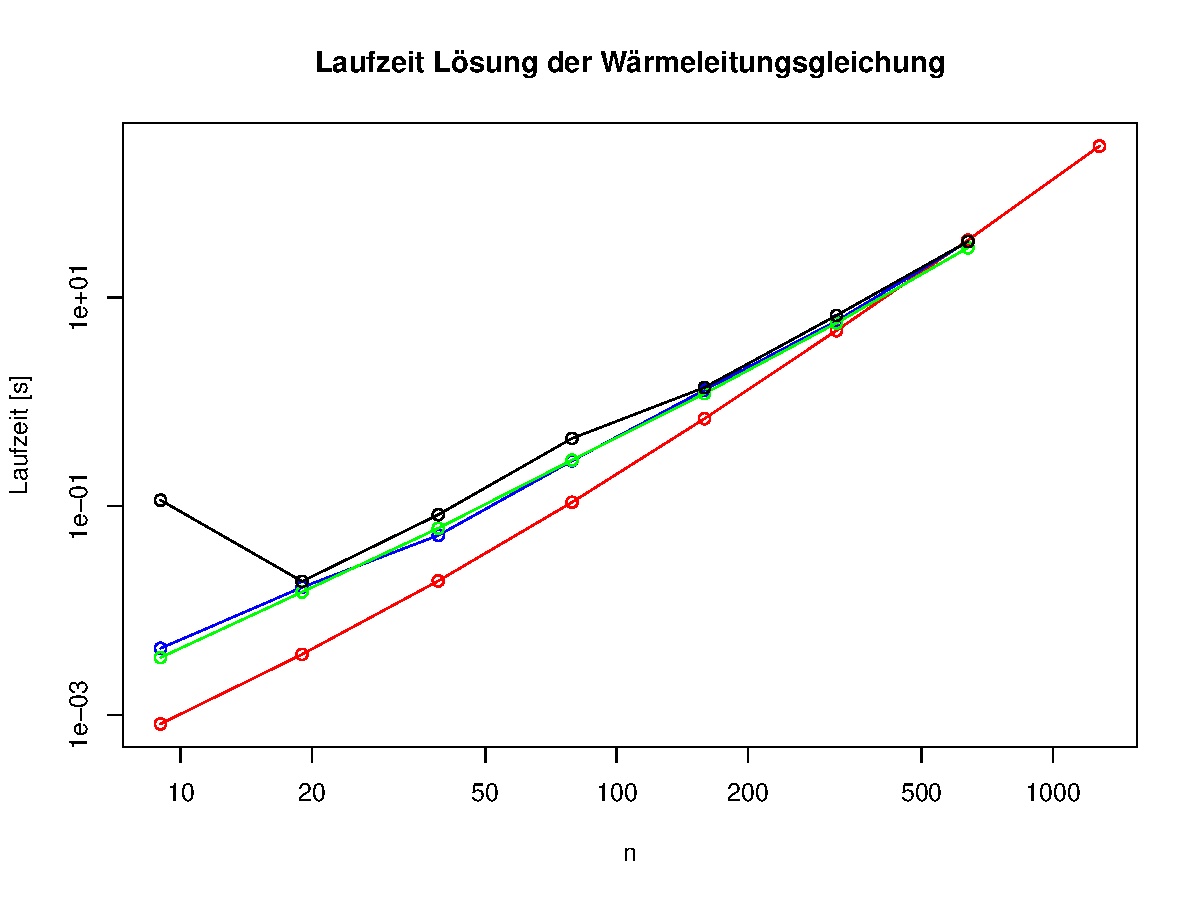
\includegraphics[width=\hsize]{heat/results-heat.pdf}
\end{center}
\caption{Laufzeit der mit OpenMP parallelisierten L"osung der
W"armeleitungsgleichung. Laufzeit mit einem einzelnen Thread ist rot
dargestellt.
\label{heat:laufzeit}}
\end{figure}

\subsection{OpenMPI}
Die Implementation mit OpenMP hat gezeigt, dass im eindimensionalen Fall
das Teilproblem zu klein ist, als dass die Parallelisierung des
Iterationsalgorithmus eine Laufzeitverbesserung ergeben k"onnte.
Das eindimensionale Problem wird also f"ur kleine $n$ am besten von einem
einzigen Prozessor gel"ost. 
Die Arbeit, die jeder Prozessor bis zum n"achsten Barrierepunkt
leistet, ist von der Gr"ossenordnung $O(n)$. 

Wenn eine parallele Implementation der L"osung der W"armeleitungsgleichung
eine bessere Laufzeit gegen"uber einer sequenziellen Implementation 
zeigen soll, dann muss die Menge der Arbeit, zwischen Barriere-Punkten
vergr"ossert werden.
Nur ein zwei- oder dreidimensionales W"armeleitungsproblem kann diese
Bedingung erf"ullen:
die Arbeit zwischen Barrierepunkten w"achst dann mit $O(n^2)$ bzw.~$O(n^3)$.

Die zweidimensionale W"armeleitungsgleichung
\[
\frac{\partial u}{\partial t}
=
\frac{\partial^2 u}{\partial x^2}
+
\frac{\partial^2 u}{\partial y^2}
\]
kann analog zur eindimensionalen W"armeleitungsgleichung diskretisiert
werden.
Die Funktion $u(t,x,y)$ wird ersetzt durch Variablen $u_{ijk}=u(ih_t,jh,kh)$.
Die zweiten partiellen Ableitungen nach $x$ und $y$ werden approximiert
werden (siehe auch Abbildung~\ref{heat:diskretisation2})
\begin{align*}
\frac{\partial^2u}{\partial x^2}
+
\frac{\partial^2u}{\partial y^2}
&
\simeq
\frac1{h^2}(
u_{i,j-1,k}-2u_{ijk}+u_{i,j+1,k}
)
+
\frac1{h^2}(
u_{i,j,k-1}-2u_{ijk}+u_{i,j,k+1}
)
\\
&=\frac1{h^2}(
u_{i,j-1,k}
+
u_{i,j,k-1}
+
u_{i,j+1,k}
+
u_{i,j,k+1}
-
4u_{ijk}
)
\end{align*}
F"ur diesen Operator wurde bereits fr"uher die Matrix $A$ in
(\ref{algorithm:laplace}) gefunden, die wir in "Ubereinstimmung mit
(\ref{heat:zerlegung}) wieder mit $N$ bezeichnen.
Dann wird die Iterationsformel wieder die gleiche Form haben wie
(\ref{heat:iteration}).
\begin{figure}
\begin{center}
\includegraphics[width=0.70\hsize]{heat/heat-2.pdf}
\end{center}
\caption{Approximation f"ur den Laplace-Operator $\Delta u$ im Punkt $(i,j)$
\label{heat:diskretisation2}}
\end{figure}

\begin{satz}
Das Iterationsverfahren (\ref{heat:iteration}) f"ur die zweidimensionale
W"armeleitungsgleichung konvergiert, wenn 
\begin{align*}
8\frac{h_t}{2h_x^2}&<1
&&\Leftrightarrow
&
h_t&<\frac{h_x^2}{4}.
\end{align*}
\end{satz}

\begin{figure}
\begin{center}
\includegraphics[width=0.8\hsize]{heat/heat-3.pdf}
\end{center}
\caption{Unterteilung des Definitionsbereiches in Teilbereiche (grau)
f"ur jeden OpenMPI Rang $r$, $0\le r<n_xn_y$.
Die d"unn ausgezogenen Rechtecke beinhalten Werte, die vor jedem 
Iterationsschritt ausgetauscht werden m"ussen.
\label{heat:domainpartition}}
\end{figure}

Zur Parallelisierung und Verteilung auf verschiedene Prozesse kann
der Definitionsbereich in $n_x$ Rechtecke in horizontaler Richtung
und $n_y$ Rechtecke in vertikaler Richtung zerlegt werden
(Abbildung~\ref{heat:domainpartition}).
Alle Teilrechtecke haben jeweils ungef"ahr die gleiche Gr"osse.
F"ur jedes Teilrechteck ist ein eigener OpenMPI Prozess zust"andig.

F"ur die Durchf"uhrung des Iterationsschrittes werden entlang des Randes
eines Teilrechtecks jeweils
die Variablen von den R"andern der Nachbarrechtecke ben"otigt.
Nach jedem Iterationsschritt m"ussen diese Werte zwischen den einzelnen
Prozessen ausgetauscht werden.
Beim Austausch fliessen die Daten in beiden Richtungen.
Da alle Prozesse sowohl Daten versenden wie auch empfangen, besteht
die Gefahr von Deadlocks: zwei Prozesse k"onnten beide auf Input warten.

Die Funktion
\verb+MPI_Send+ blockiert, bis die Daten im Zielprozess angekommen sind.
Daher wurde in der Implementation die Funktion \verb+MPI_Isend+ verwendet,
welche sofort zur"uckkommt. Alle Prozesse kopieren ihre Randdaten in
einen Sende-Puffer, und "ubermitteln ihn mit \verb+MPI_Isend+.
Danach k"onnen alle Prozesse die Rand-Daten in beliebiger Reihenfolge
empfangen, womit Deadlocks vorgebeugt wird.
Wenn die Empfangs-Funktionen (\verb+MPI_Recv+) abgeschlossen sind,
dann sind auch die Sende-Operationen fertig.

Abbildung \ref{heat:threadzahl} zeigt die Abh"angigkeit der Laufzeit von der
Threadzahl f"ur ein Problem der Gr"osse $n=2560 \times 1440=3686400$.
F"ur einen einzelnen Iterationsschritt, also zwischen zwei Austauschschritten
f"ur die Randwerte m"ussen bei 4 Prozessen in jedem Prozess fast eine Million
Variablen neu berechnet werden, was mindestens 6 Rechenoperationen erfordert.
Damit ist sichergestellt, dass die reine Rechenzeit in den Iterationsschritten
die Gesamtzeit dominiert, was sich auch in der guten Skalierung bis
zur Gesamtzahl der Prozesse zeigt.

\begin{figure}
\begin{center}
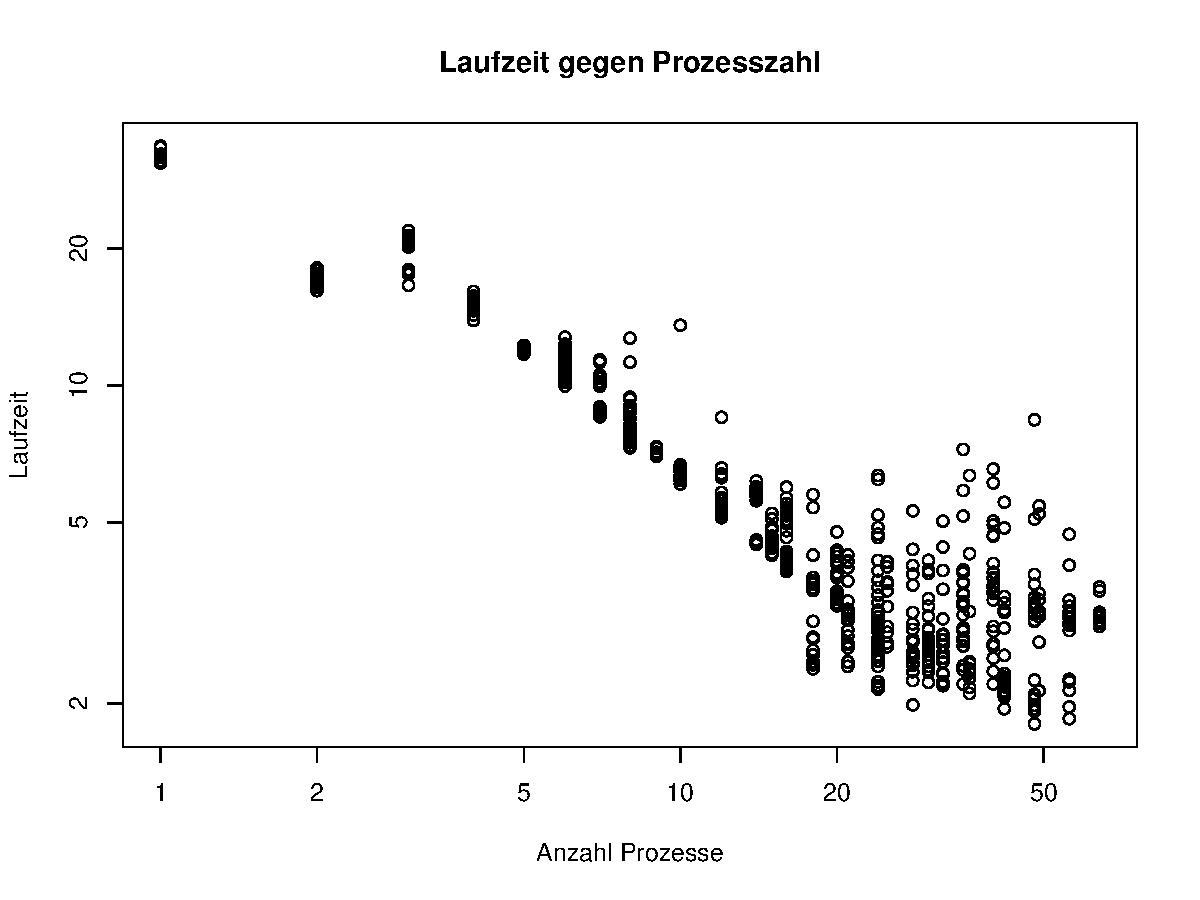
\includegraphics[width=\hsize]{heat/results-heat-threads.pdf}
\end{center}
\caption{Laufzeit der mit OpenMPI parallelisierten L"osung der
W"armeleitungsgleichung in Abh"angigkeit von der Prozesszahl.
Mehr als 20 Prozesse gegen auf der verwendeten 4-Prozessor-Maschine
keine verbesserte Laufzeit, und die durch stochastischen
Overhead verursachte Streuung dominiert die Laufzeit.
\label{heat:threadzahl}}
\end{figure}

\subsection{Visualisierung der Resultate}
Die Funktion $u(x,y)$ kann als Bild visualisiert werden.
Das Beispielprogramm hat daher Kommando\-zeilen-Optionen, mit welchen man
verlangen kann, dass $u(x,y)$ f"ur jeden Zeitpunkt als FITS-Bild
gespeichert werden. Diese Bilder kann man dann in JPEG-Bilder konvertierung
und in MPEG-Video codieren.
\begin{figure}
\begin{center}
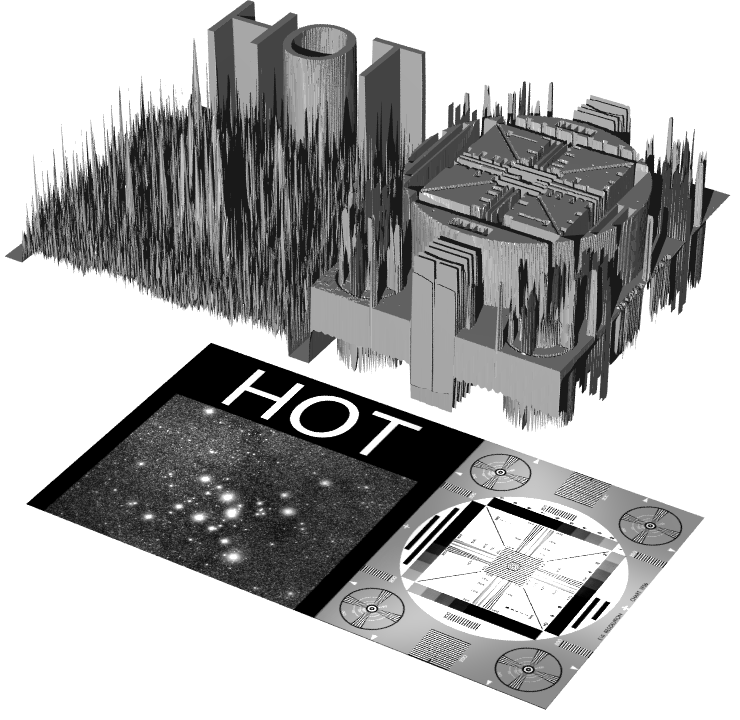
\includegraphics[width=\hsize]{heat/heat-i00000.png}
\end{center}
\caption{Darstellung der L"osung der W"armeleitungsgleichung
f"ur $t=0$.
\label{heat:t0}}
\end{figure}
%
\begin{figure}
\begin{center}
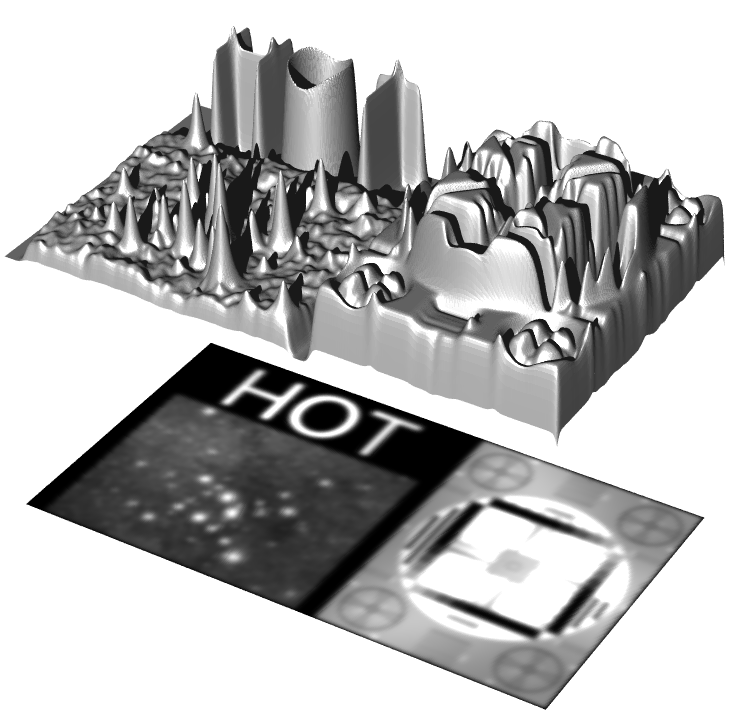
\includegraphics[width=\hsize]{heat/heat-i00025.png}
\end{center}
\caption{Darstellung der L"osung der W"armeleitungsgleichung
f"ur $t=25$.
\label{heat:t25}}
\end{figure}
%
\begin{figure}
\begin{center}
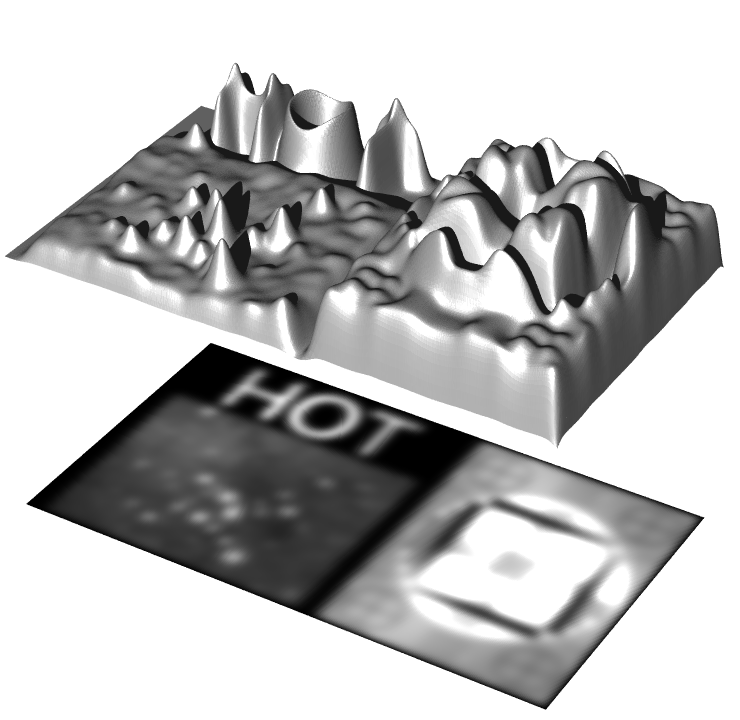
\includegraphics[width=\hsize]{heat/heat-i00100.png}
\end{center}
\caption{Darstellung der L"osung der W"armeleitungsgleichung
f"ur $t=100$.
\label{heat:t100}}
\end{figure}
%
\begin{figure}
\begin{center}
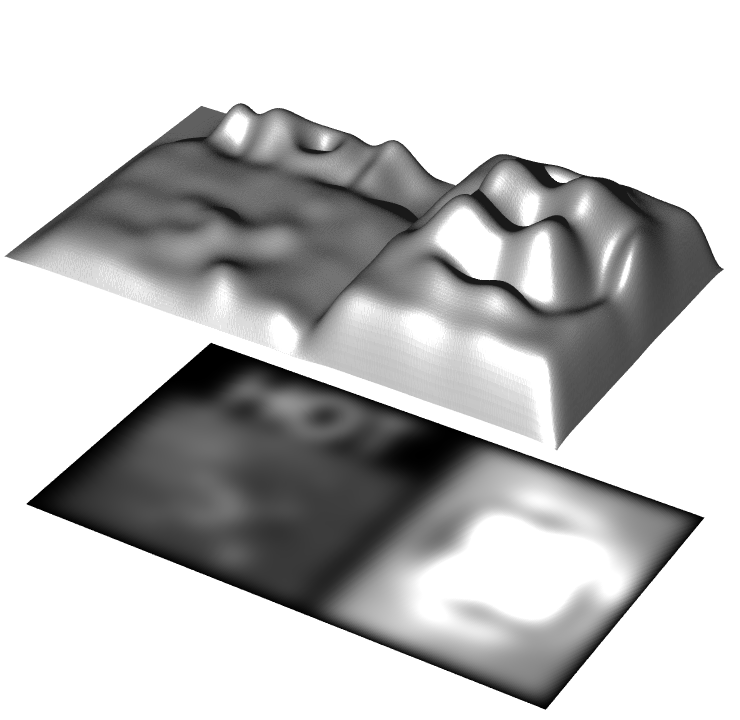
\includegraphics[width=\hsize]{heat/heat-i00500.png}
\end{center}
\caption{Darstellung der L"osung der W"armeleitungsgleichung
f"ur $t=500$.
\label{heat:t500}}
\end{figure}

Gew"ohnlich werden Funktionen von zwei Variablen auch als Fl"achen "uber
dem Definitionsbereich dargestellt.
Als Beispiel f"ur eine solche Darstellung wurde das Programm {\tt fits2pov} 
hinzugef"ugt, welches ein FITS-Bild in eine Fl"achenbeschreibung f"ur
das Ray-Tracing-Programm Povray umwandelt. Povray kann dann verwendet
werden, die Fl"ache ebenso wie das urspr"ungliche Bild als 3D-Bild
darzustellen, und die JPEG-Bilder wieder als MPEG-Video zu kodieren.
Die Abbildungen \ref{heat:t0} bis \ref{heat:t500} zeigen einzelne Bilder
aus diesem Video.
Abbildung~\ref{heat:t0} zeigt die Anfangsbedingung zur Zeit $t=0$.
Als Zeitskala wird die Anzahl Zeitschritte verwendet, in einer Simulation
aus einem Gitter mit $640\times 360$ Gitterpunkten.
Bereits nach 25 Schritten sind alle scharfen Kanten in der Anfangsbedingung
verschwunden.
In Abbildung~\ref{heat:t100} kann man gut sehen, wie die scharfen
Peaks der Anfangsbedingung bei den Sternen zu zweidimensionalen
Gauss-Verteilungen geworden sind, wie die elementare L"osung
(\ref{heat:solution}) erwarten l"asst.

\begin{aufgabe}
Man simuliere die Bewegung der Sterne in einem Kugelsternhaufen.
\end{aufgabe}

Wikipedia:
\begin{quote}
Ein Kugelsternhaufen (kurz auch Kugelhaufen) ist eine enge,
kugel\-f"ormige Ansammlung sehr vieler Sterne, die untereinander
gravitativ gebunden sind. Typische Gr"ossen sind einige 100000 Sterne.
Gegenseitige Bahnver"anderungen sind im dicht bev"olkerten Zentrum
h"aufig, was die sph"arische Gestalt zur Folge hat. Kugelsternhaufen
sind ihrerseits gravitativ an Galaxien gebunden, in deren Halo sie
sich weitr"aumig bewegen. Sie bestehen vorwiegend aus alten, roten
Sternen, die nur wenige schwere Elemente enthalten.
\end{quote}

Ziel dieser Aufgabe ist eine Simulation der Bewegung der Sterne in
einem Kugelsternhaufen durchzuf"uhren. Dabei k"onnten folgende Fragen
von Interesse sein:
\begin{enumerate}
\item Wie h"angt die Sterndichte nahe dem Zentrum des Kugelsternhaufens
von der Zeit ab?
\item Wie lange dauert es, bis der Kugelsternhaufen einen stabilen
Radius gefunden hat?
\item Wie h"aufig kommt es vor, dass Sterne aus dem Kugelsternhaufen
ausgestossen werden?
\item Wie "andert ein schwarzes Loch mit 20000 Sonnenmassen im Zentrum
eines Kugelsternhaufens die Antworten zu obigen Fragen?
\end{enumerate}

\begin{aufgabe}
Str"omungssimulation mit OpenFOAM.
\end{aufgabe}

OpenFOAM ist ein Open Source Softwarepaket zur Str"omungssimulation.
Ziel dieser Aufgabe ist darzulegen, wie ein erfolgreiches Produkt
wie OpenFOAM die verschiedenen Techniken einsetzt, die im 
Vorlesungsteil besprochen worden sind.

Als Basis f"ur diese Diskussion soll ein einfaches Str"omungsproblem
gel"ost werden.
Es soll die Str"omung um einen Fl"ugel mit einem sehr flachen Rhombus
als Querschnitt berechnet werden. 
Folgende Fragen k"onnten dabei von Interesse sein:
\begin{enumerate}
\item Wie h"angen Auftrieb und Widerstand vom Anstellwinkel ab?
\item Bei welchem Anstellwinkel beginnt sich die Str"omung abzul"osen?
\end{enumerate}


\begin{aufgabe}
Google hat f"ur Big-Data Anwendungen das Map-Reduce Paradigma
eingef"uhrt.
Hadoop ist eine beliebte Java-Implementation von Map-Reduce.
Map-Reduce ist in erster Linie auf (einfachen) Operationen auf 
grossen Datenmengen ausgelegt, w"ahrend in HPC eher die Menge der
Operationen das Problem ist.
\begin{itemize}
\item Gibt es Beispiele die Anwendung von Map Reduce und Hadoop f"ur
HPC Probleme?
\item Wie Verwendet man MapReduce/Hadoop an einem konkreten Beispiel?
\item Wie gross ist der Overhead, wie gut skaliert eine Map-Reduce L"osung?
\end{itemize}
\end{aufgabe}

M"oglicher Einstiegspunkt in die Literatur:
\begin{itemize}
\item
\url{http://de.slideshare.net/dgleich/mapreduce-for-scientific-simulation-analysis} 
\item
\url{http://de.slideshare.net/dgleich/tallandskinny-qr-factorizations-in-mapreduce-architectures}.
\item
\url{http://dimacs.rutgers.edu/Workshops/Parallel/slides/muthu.pdf}
\end{itemize}


\begin{aufgabe}
Die Monte-Carlo Methode.
\end{aufgabe}

Probabilistische Algorithmen k"onnen deterministische Probleme l"osen,
insbesondere wenn keine direkten deterministischen Algorithmen bekannt 
sind.
Um eine vergleichbare Genauigkeit mit traditionellen Algorithmen zu
erreichen, ist eine sehr viel gr"ossere Zahl von Einzelresultaten notwendig.

Ein einfaches Beispiel f"ur einen Monte-Carlo Algorithmus ist die Integration
einer Funktion $f\colon[0,1]\to[1,0]$.
Statt das Integral direkt zu berechnen,
bestimmt man empirisch die Wahrscheinlichkeit, dass $P(Y < f(X))$, wobei
$X$ und $Y$ in $[0,1]$ gleichverteilte Zufallsvariablen sind. Dann gilt
\[
P(Y<f(X)) = \int_0^1f(x)\,dx.
\]
Eine Schwierigkeit bei der Durchf"uhrung einer Monte-Carlo-Simulation
ist, eine Quelle gen"ugend zuf"alliger Zufallszahlen zu bekommen.
Inbesondere hat man in Graphikkarten a priori keine guten
Zufallszahlgeneratoren. 

Ein alternatives Problem, welches man mit Monte-Carlo-Simulation untersuchen
k"onnte, handelt von der Akkumulation von Fehlern in einer Tr"agheitsplattform.
Eine solche muss zu Beginn auserichtet werden, was nat"urlich nicht
exakt m"oglich ist. Die Orientierung einer Tr"agheitsplattform wird gegeben
durch eine orthogonale Matrix in $\operatorname{SO}(3)$. 
Die tats"achliche Orientierung einer Tr"agheitsplattform ist also eine
Wahrscheinlichkeitsdichte auf $\operatorname{SO}(3)$, sie ordnet jeder m"oglichen
Orientierung eine gewisse Wahrscheinlichkeit zu.

Im Betrieb "andert sich die Orientierung der Plattform, durch Messung
der Winkelgeschwindigkeit kann man die wahrscheinlichste Orientierung
berechnen.
Unvermeidliche Messfehler der drei Winkelgeschwindigkeitssensoren
f"uhren aber dazu, dass die Ungenauigkeit immer gr"osser wird, die
Wahrscheinlichkeitsverteilung auf $\operatorname{SO}(3)$ wird immer ``verwaschener''.
Es gibt eine Vermutung, dass dies von einer Art Diffusions- oder
W"armeleitungsgleichung beschrieben wird.
Eine interessante Anwendung von Monte-Carlo-Simulation w"are, die
Entwicklung der Verteilung damit zu berechnen, und mit der 
Differentialgleichung zu vergleichen.

Historische Aspekte zur Monte-Carlo-Method:
\url{http://library.lanl.gov/cgi-bin/getfile?00326866.pdf}

\begin{aufgabe}
Ising-Modell
\end{aufgabe}

Das Ising-Modell beschreibt einen Ferromagneten, bestehend aus 
Spins $S_i$, die in einem Gitter angeordnet sind. Die Energie
in ist gegeben durch
\[
H(S)=-J\sum_{\text{$i,j$ benachbart}}S_iS_j + B\sum_i S_i
\]
Die Statistische Mechanik liefert einen Formalismus, wie man thermodynamische
Eigenschaften dieses Systems berechnen kann. Dazu muss man die Zustandssumme
\[
Z_\beta = \sum e^{-\beta S}
\]
berechnen, wobei $\beta=1/k_BT$ die inverse Temperatur ist.
Die Summe erstreckt sich "uber alle m"oglichen Zust"ande, und genau das
ist das Problem: ein $100\times 100 \times 100$ Gitter, also immer noch
ein sehr kleiner Kristall, hat $2^{100^3}\simeq 10^{301029}$ Zust"ande,
diese Summe kann also praktisch nicht berechnet werden.

Eine Simulation ist n"otig.
Es existiert eine Reihe von Algorithmen, mit denen ein Gleichgewichtszustand
gefunden werden kann.
W"ahlen Sie einen Algorithmus und implementieren Sie eine parallelisierte
Version desselben.

\begin{itemize}
\item
\url{http://en.wikipedia.org/wiki/Ising_model}
\item
\url{http://www.comphys.ethz.ch/hans/p/047.pdf}
\item
\url{http://physics.unifr.ch/admin/dbproxy.php?table=fuman_filepool&column=content&id=1267}
\end{itemize}



\section{Voraussetzungen}

\section{Bewertung}
\subsection{Note}
Die Vortr"age und Papers werden benotet und geben die Modulnote.
Die Note setzt sich zusammen aus den Resultaten eines Fragebogens,
den die Zuh"orer ausf"ullen, und einer Benotung durch den Dozenten.

\subsection{Kurztests}
Ausserdem werden drei Kurztests durchgef"uhrt, die nur bestanden
werden k"onnen oder nicht. 
{\em Nichtlineare Optimierung} und {\em Variationsrechnung} je
ein Kurztest bestehend aus einer Standardaufgabe aus den jeweiligen
Themengebieten verlangt. In diesem Kurztest d"urfen beliebige Hilfsmittel
verwendet werden, auch Computer und das Internet, und es gibt keine
Zeitlimite (ausser der Schliessung des Ge"audes).

Mit dem Kurztest
soll bewiesen werden, dass jeder Teilnehmer mit den grundlegenden
Techniken des HPC vertraut ist.
Die Kurztests geben keine Note, m"ussen aber alle erf"ullt sein,
damit das Modul als bestanden gilt.

\end{document}
 
